\documentclass[11pt]{article}
%基于北京航空航天大学仪器科学与光电工程学院实验报告及课程报告排版得来,类似于毕业论文排版格式
%后续将更新毕业论文排版格式
\usepackage{graphicx,float}%使用图的宏包,使用图的浮动体宏包,引入参数H使图像紧跟当前文字
\usepackage{caption} %使用图表标题的宏包
\usepackage[colorlinks=true,pdfstartview=FitH,%
linkcolor=black,anchorcolor=violet,citecolor=magenta]{hyperref}%加载hyperref宏包,使用超链接
\usepackage{setspace}%用于设置行间距列间距等命令的宏包
\usepackage{array}%设置列表高度宽度的宏包
\usepackage{zhnumber}%使用中文数字编号的宏包
\usepackage{titlesec,titletoc}%使用标题自定义形式的宏包和使用目录自定义形式的宏包
\usepackage{siunitx}%物理学单位宏包
\usepackage{tabularx}%让表格宽度等于页面宽度
\usepackage{makecell}%单个表格单元调整的宏包
\usepackage{subfigure} %%使用子图的宏包
\usepackage[backend=biber,bibstyle=gb7714-2015,%nature,%%加载biblatex宏包,使用参考文献
citestyle=gb7714-2015%,backref=true%%其中后端backend使用biber
,url=false,doi=false
]{biblatex}%标注(引用)样式citestyle,著录样式bibstyle都采用gb7714-2015样式
% \usepackage{pgfplots}%类似tikz的一个画图库,主要画统计图
\usepackage{../customStyle}
% \usepackage{customFont}%自行编写的字体命令库,基于CJK宏包
% \usepackage{bh_style}%自行编写的风格文件,基于使用习惯和格式要求
% \usepackage{math_formulate}%自行编写的数学公式命令库,基于amsmath宏包
% \usepackage{picture}%集成图形绘制库,主要包括了tikz和pgfplots两大主流宏包
% \usepackage[lite,subscriptcorrection,slantedGreek,nofontinfo]{mtpro2}%使用mathtimepro2商业字体作为数学环境,并不推荐

%biblatex宏包的参考文献数据源加载方式,注意book.bib应当与.tex文件在同一目录下,不然有可能会报错
\addbibresource[location=local]{book.bib}
% % \bibliographystyle{gbt7714-numerical}
%%% 下面的命令重定义页面边距,使其符合中文刊物习惯 %%%%
% \addtolength{\topmargin}{2.5cm}
\setlength{\oddsidemargin}{0.63cm}  % 3.17cm - 1 inch
\setlength{\evensidemargin}{\oddsidemargin}
% \setlength{\textwidth}{14.66cm}
% \setlength{\textheight}{24.00cm}    % 24.62

\graphicspath{{./fig}}

\begin{document}
{
  %% ----------- 封面部分 ------------ %%
\pagestyle{empty}
\begin{figure}
  
\includegraphics{title.jpg}
\end{figure}
\begin{center}

  \begin{figure}[h]

    \centering
    
\includegraphics[]{title.png}\par
    \vspace{4em}
    \large{\chuhao\heiti{机电仿真实验}}\par
    \vspace{6em}
  \end{figure}

  
  \large{\yihao\heiti{Labwindows/CVI实验报告}}\par
  \vspace{8em}

  \begin{spacing}{2.0}
    \begin{tabular}{cc}


      {\xiaosanhao\heiti{学\quad 院\quad 名\quad 称}} & {\xiaosanhao\heiti{\dlmu{仪器科学与光电工程学院}}}    \\
      {\xiaosanhao\heiti{学\quad \quad\quad\quad\quad 号}} & {\xiaosanhao\heiti{\dlmu{SY2317301} }} \\
      {\xiaosanhao\heiti{姓\quad \quad\quad\quad\quad 名}} & {\xiaosanhao\heiti{\dlmu{陈博非} }}       \\
    \end{tabular}
  \end{spacing}
\end{center}
\begin{center}
  {\xiaoerhao\heiti{\now}}
\end{center}

\thispagestyle{empty}
}

\newpage
%% ----------- 封面部分结束 ------------ %%


%% ----------- 目录部分 ------------ %%
% \pagenumbering{roman}

% \setcounter{tocdepth}{3}
% %设定目录深度                      
% \tableofcontents
% %列出目录
% \newpage
%% ----------- 目录部分结束 ------------ %%
\pagenumbering{arabic}
\setcounter{page}{1}

\section{背景介绍}

\section{技术方案}
% \begin{figure}[H]
%   \centering
%   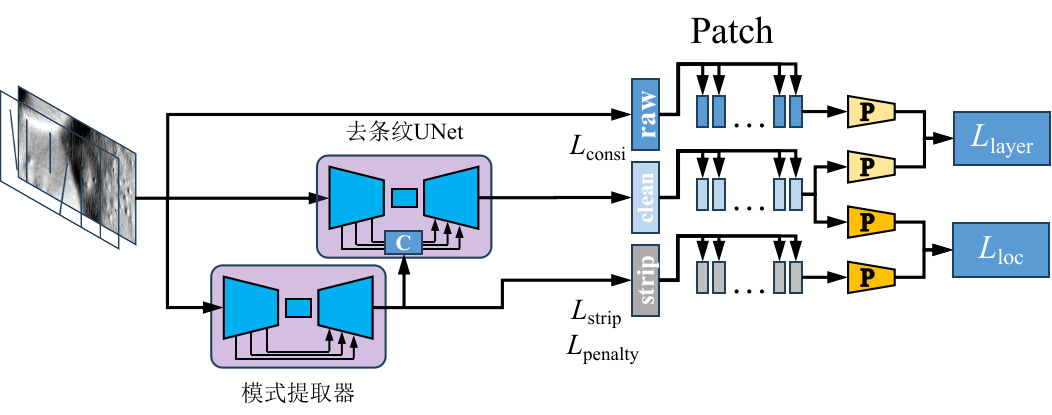
\includegraphics[width=0.8\textwidth]{workflow.png}
%   \caption{检测算法工作流程}
%   \label{fig:workflow}
% \end{figure}
下面简要地介绍各个部分的工作过程。
\subsection{数据加载环节}

\subsection{扩散网络环节}

\subsection{后处理环节}

\section{算法原理}

\section{程序设计流程与说明}

\section{实验结果与分析}

\section{结论}

\newpage
\printbibliography[heading=bibliography,title=参考文献]
\end{document}
